\documentclass[12pt,a4paper]{report}

% ---------- Packages ----------
\usepackage[utf8]{inputenc}
\usepackage[T1]{fontenc}
\usepackage{geometry}
\geometry{a4paper, margin=1in}
\usepackage{titlesec}
\usepackage{graphicx}
\usepackage{booktabs}
\usepackage{longtable}
\usepackage{array}
\usepackage{xcolor}
\usepackage{enumitem}
\usepackage{hyperref}
\usepackage{fancyhdr}
\usepackage{tikz}
\usetikzlibrary{shapes,arrows.meta,positioning}
\usepackage{caption}

\hypersetup{
    colorlinks=true,
    linkcolor=black,
    citecolor=black,
    urlcolor=blue
}

\pagestyle{fancy}
\fancyhf{}
\fancyhead[L]{FoodBridge}
\fancyhead[R]{\thepage}
\renewcommand{\headrulewidth}{0.4pt}

% ---------- Diagram placeholder command ----------
% Usage: \diagramplaceholder{width}{height}{Caption text}
\newcommand{\diagramplaceholder}[3]{%
\begin{figure}[h!]
\centering
\fbox{%
  \begin{minipage}[c][#2][c]{#1}
    \centering
    \color{gray}\textit{[Insert diagram here: #3]}
  \end{minipage}%
}
\caption{#3}
\end{figure}
}

\title{}
\date{}

\begin{document}

% ================= TITLE PAGE =================
\begin{titlepage}
\centering
\vspace*{1cm}
{\Large \textbf{UCS503P -- Software Engineering Lab}}\\[1.5cm]

{\Huge \textbf{FoodBridge}}\\[0.5cm]
{\Large A Surplus Food Redistribution Matcher}\\[2cm]

{\large \textbf{Submitted by:}}\\[0.3cm]
1024030119 \quad Hardik Pajiala\\
1024030916 \quad Shikhar Goel\\
1024030164 \quad Aayush Shukla\\[0.6cm]
Group: 3, BE Third Year, Computer Engineering\\[1.5cm]

{\large \textbf{Submitted to:}}\\[0.3cm]
Ms. Anushka\\[1.5cm]
{\large \textbf{Prototype Report / Mid-Semester Evaluation}}\\[0.5cm]

\vfill

Computer Science and Engineering Department\\
Thapar Institute of Engineering and Technology, Patiala

\end{titlepage}

% ================= TOC =================
\tableofcontents
\clearpage

% ================================================================
\chapter{Introduction}

\section{Background and Context}

Restaurants, hostel and institutional mess halls, caterers, and event organisers routinely generate surplus edible food, while nearby welfare organisations, shelters, and community kitchens struggle to source food on short notice. The food is safe and immediately consumable, but only within a short and shrinking window. FoodBridge aims to reduce avoidable food waste in urban settings by shortening the coordination gap between organisations that generate surplus edible food and welfare organisations that can consume it within its usable window.

While the topic touches on broader questions of food security and sustainability, the immediate engineering objective is narrower and concrete: to translate an informal, phone-and-messaging-based redistribution practice into a measurable, deployable software workflow in which allocation decisions are recorded, reviewable, and made against explicit criteria.

The binding constraint is time, not willingness. A donation typically has a usable window of a few hours; a coordination process that consumes most of that window converts a solvable logistics problem into waste. Even modest reductions in time-to-match therefore translate directly into food that is eaten rather than discarded.

\subsection{Problem Statement}

Today's informal redistribution practice suffers from four recurring pain points:

\begin{itemize}[leftmargin=*]
    \item \textbf{Fragmentation:} availability is announced through calls, messaging groups, and personal contacts, so surplus arising outside a coordinator's existing network is never discovered at all.
    \item \textbf{Unoptimised allocation:} where a listing does reach several organisations, the food goes to whoever replies first. Response speed correlates with volunteer availability, not with proximity, need, or the donation's remaining shelf life.
    \item \textbf{Low transparency:} a donor who hands food over has no record of whether it was collected or wasted, and a recipient has no visibility of what is available nearby right now.
    \item \textbf{No measurement:} because nothing is recorded, neither party can establish what was redistributed, and no baseline exists against which any improvement could be claimed.
\end{itemize}

\section{Project Objectives}

\begin{enumerate}[leftmargin=*]
    \item \textbf{Objective 1:} Deliver an end-to-end donation workflow --- post, review, match, collect, confirm --- with the simplest allocation rule that works, so that a working system exists from the first iteration.
    \item \textbf{Objective 2:} Reduce the median Time-to-Match (TTM) between donation submission and an accepted match to $\leq$ 20 minutes, measured purely from database timestamps rather than self-report.
    \item \textbf{Objective 3:} Make every allocation decision explainable and improvable by isolating the matching logic behind a stable service interface, first as a greedy best-fit assignment and later upgraded to a global assignment using the Hungarian method, without disrupting the rest of the system.
\end{enumerate}

These objectives are Specific, Measurable, Achievable, Relevant, and Time-bound: each is tied to a concrete deliverable or a timestamp-derived metric. Chapter 3 reports the status of each against the working prototype.

% ================================================================
\chapter{Methodology and Design}

\section{System Architecture}

\subsection{High-Level Design}

FoodBridge is a web-based ``Surplus-to-Recipient'' matching system built from five cooperating components:

\begin{itemize}[leftmargin=*]
    \item \textbf{Donor submission portal:} a donor posts a surplus listing with food type, quantity in servings, expiry/pickup deadline, and pickup location.
    \item \textbf{Recipient registration:} welfare organisations register with their service area, serving capacity, and food-type constraints.
    \item \textbf{Administrative review:} an administrator approves or rejects each submitted donation before it becomes eligible for matching, so that an illegitimate or unusable listing never reaches an organisation.
    \item \textbf{Automated matching:} the system filters organisations that cannot accept the donation and ranks the remainder on proximity, urgency, and capacity fit, then offers the donation to the best-fit organisation rather than broadcasting it.
    \item \textbf{Status transparency and impact reporting:} both parties track the donation through its lifecycle and are notified at each transition, and an administrative dashboard summarises servings redistributed, median time-to-match, and donations lost to expiry.
\end{itemize}

\begin{figure}[h!]
\centering
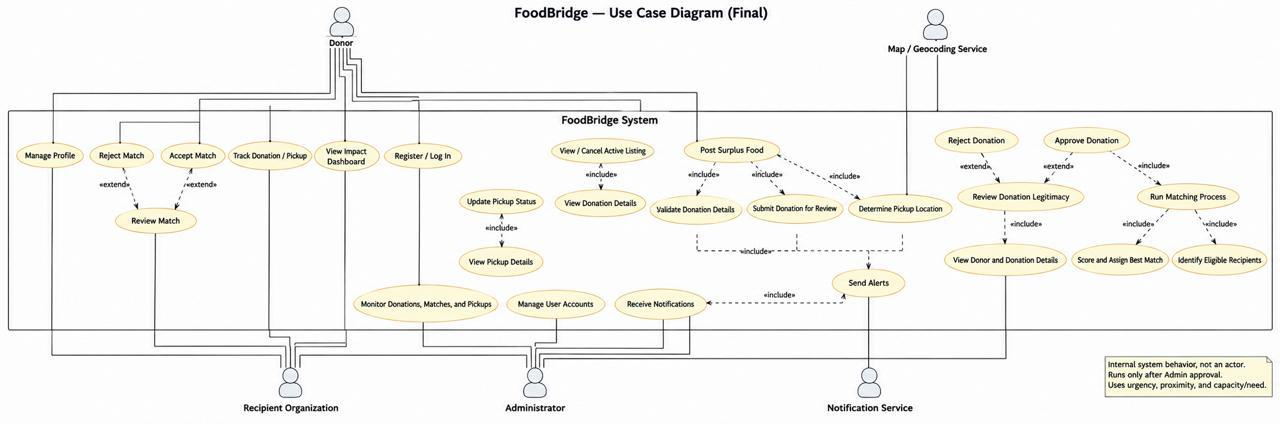
\includegraphics[width=\textwidth]{images/usecase.jpeg}
\caption{Use case diagram: actors and system interactions}
\label{fig:usecase}
\end{figure}

\subsection{Donation Lifecycle}

The workflow enforces a fixed transition sequence, writing a system timestamp at every transition. These timestamps are the sole basis for the evaluation metrics in Chapter 4.

\begin{longtable}{@{}p{3.5cm}p{10cm}@{}}
\toprule
\textbf{State} & \textbf{Meaning} \\
\midrule
\endhead
PENDING\_REVIEW & Submitted by a donor; awaiting administrative approval. \\
POSTED & Approved and eligible for matching. \\
REJECTED & Rejected at review, with a recorded reason. \\
MATCHED & Offered to an organisation; a match record holds the offer and its score. \\
PICKED\_UP & Collected by the accepting organisation. \\
COMPLETED & Redistribution confirmed complete. \\
CANCELLED & Withdrawn by the donor before collection. \\
EXPIRED & Reached its deadline uncollected; counted against the system's own performance. \\
\bottomrule
\end{longtable}
\captionof{table}{Donation states as implemented}

Acceptance is deliberately a property of a match rather than of a donation. A donation may be offered to several organisations in sequence --- declined or timed out by one, re-offered to the next --- so the accept/decline decision belongs to the individual offer. This is why the state list above contains no separate ``Accepted'' donation state.

\begin{figure}[h!]
\centering
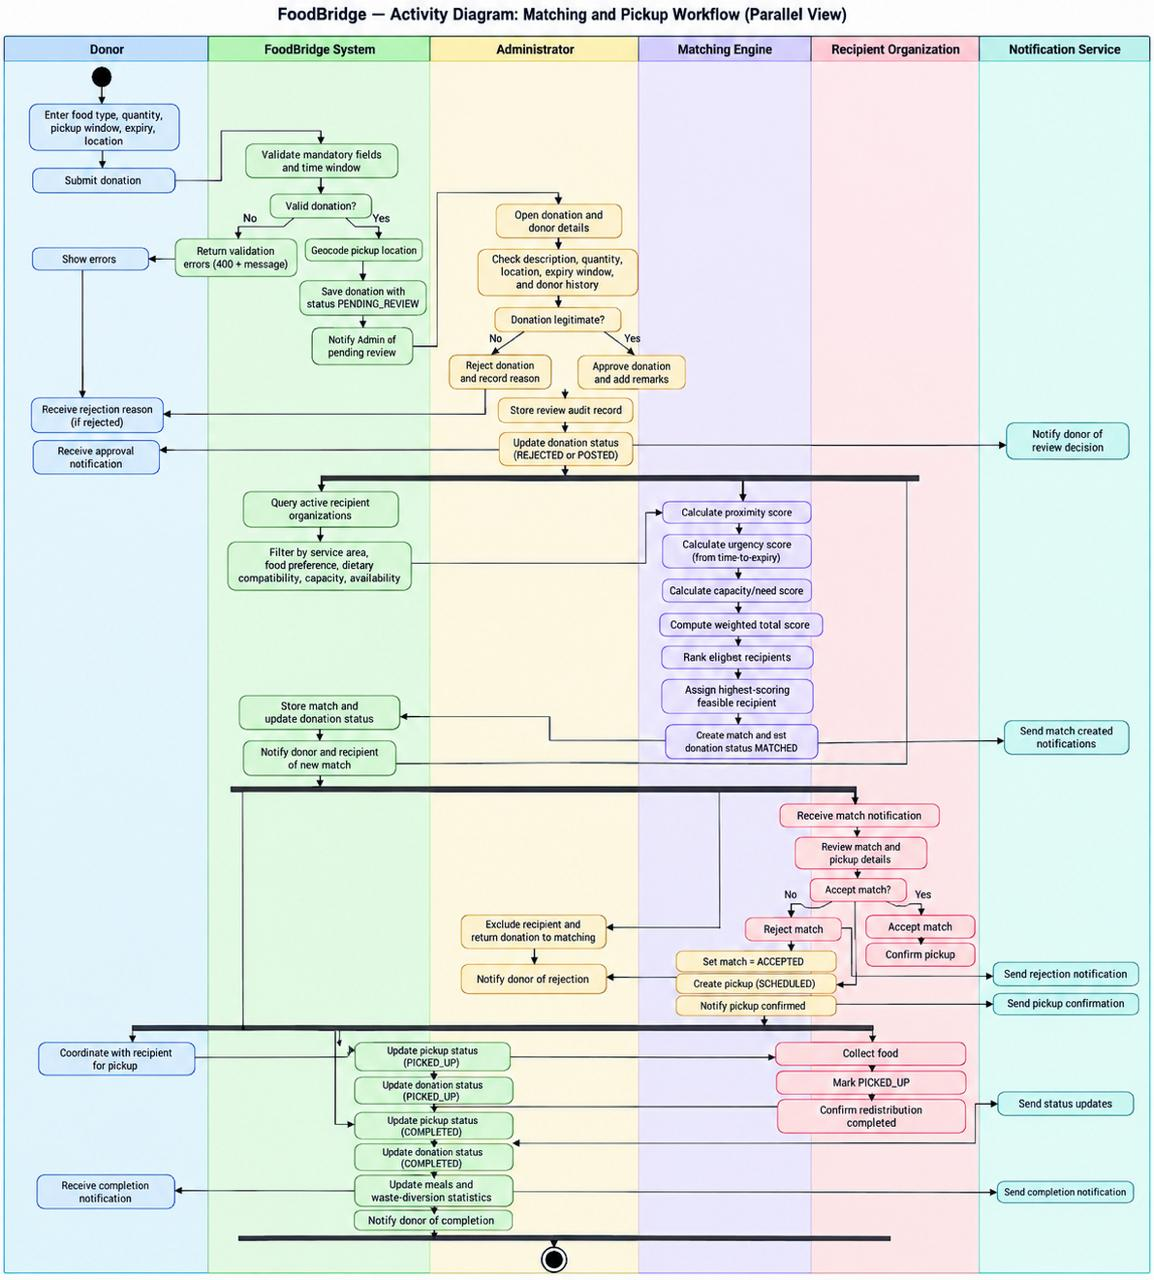
\includegraphics[width=\textwidth]{images/activity.jpeg}
\caption{Activity diagram: matching and pickup workflow (parallel view)}
\label{fig:activity}
\end{figure}

\subsection{Technical Stack}

\begin{itemize}[leftmargin=*]
    \item \textbf{Frontend:} React with Vite --- a responsive interface for donors, recipient organisations and administrators, covering authentication, the submission form, the match inbox, the status timeline, and the impact dashboard.
    \item \textbf{Backend API:} Node.js with Express, written in TypeScript, handling authentication, submission, geocoding, administrative review, status transitions, re-match on decline, and notification dispatch.
    \item \textbf{Matching service:} a stateless Python component built with FastAPI, exposing a single operation --- given open donations and eligible organisations, return a scored assignment. It is testable in isolation with no database dependency.
    \item \textbf{Database:} PostgreSQL 17 with the PostGIS spatial extension, storing users, donors, recipient organisations, donations, matches with their score components, pickups, reviews, the matching waitlist, notifications, and a geocoding cache. GiST indexes on the geography columns support radius-constrained candidate retrieval directly in the query.
    \item \textbf{Authentication:} token-based authentication implemented in the API using JSON Web Tokens, with passwords hashed using bcrypt. Roles are carried in the token and enforced at the route level.
    \item \textbf{Tools:} Vitest for backend tests, pytest for the matching service, ESLint for the frontend, and a purpose-written contract-conformance check that verifies the API satisfies everything the client requires.
\end{itemize}

This stack was chosen deliberately from mature, well-understood components so that the team's effort goes into workflow design, correctness, and measurement rather than into building or debugging new infrastructure.

\section{Implementation Details}

\subsection{Module 1: Donation Workflow and Status Transitions}

The core functionality module owns the donation lifecycle. A donor submission generates a donation identifier and triggers geocoding; the donation then enters administrative review. On approval it becomes eligible for matching. Every transition is validated against a central state machine, so an illegal transition is rejected with a defined error rather than silently corrupting the record, and each transition writes a timestamp.

The handover is deliberately two-sided: the collecting organisation records the pickup and confirms receipt, and both events are stored on a separate pickup record with its own lifecycle. Keeping the pickup distinct from the donation means the collection has its own audit trail and its own timestamps.

\subsection{Module 2: Matching and Allocation Engine}

Allocation is built from mature, well-understood parts and is treated as one well-isolated component of the workflow system rather than as a research contribution:

\begin{itemize}[leftmargin=*]
    \item \textbf{Hard constraints as filters:} an organisation that is inactive, outside its declared service radius, or without sufficient remaining capacity is removed from consideration before any scoring occurs.
    \item \textbf{Weighted ranking:} a transparent weighted score is computed over three normalised components --- urgency (time remaining before expiry, weight 0.40), proximity (weight 0.35), and capacity fit (weight 0.25). The weights are configuration, not hidden logic, and every match stores its component values so that any allocation can be explained after the fact.
    \item \textbf{Progressive radius expansion:} matching begins at a small search radius and widens in steps up to a configured maximum. A donation that still finds no eligible organisation is placed on a waitlist and retried rather than dropped.
    \item \textbf{Greedy first iteration:} donations are processed in order of urgency and each is offered to its highest-scoring available organisation. This is simple, fast, and correct for the common case of sparsely arriving donations.
    \item \textbf{Global assignment:} a global assignment across all simultaneously open donations, using the Hungarian method via \texttt{scipy.optimize.linear\_sum\_assignment}. This is a long-established algorithm available as a standard library primitive, chosen precisely because it carries no implementation risk. Both strategies are implemented and selectable at run time.
    \item \textbf{Human decision retained:} the system offers and ranks; it never silently discards a donation or forces an assignment. Declines are treated as a normal path, not an error --- a declined offer requeues the donation and excludes the declining organisation from the next cycle.
\end{itemize}

\begin{figure}[h!]
\centering
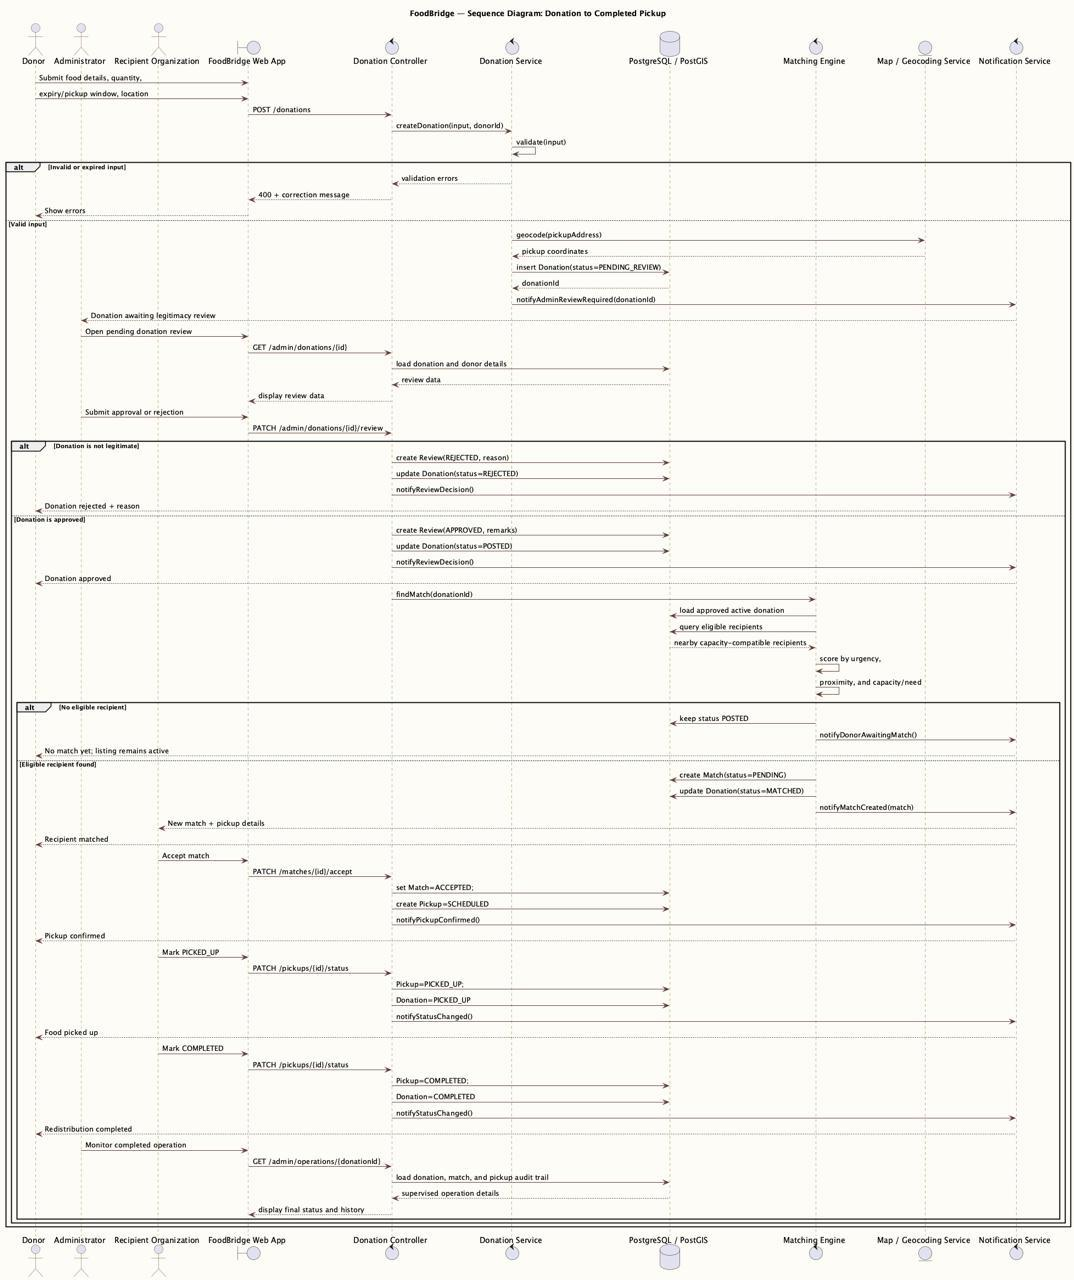
\includegraphics[width=\textwidth]{images/sequential.jpeg}
\caption{Sequence diagram: donation submission through match acceptance}
\label{fig:sequence}
\end{figure}

\begin{figure}[h!]
\centering
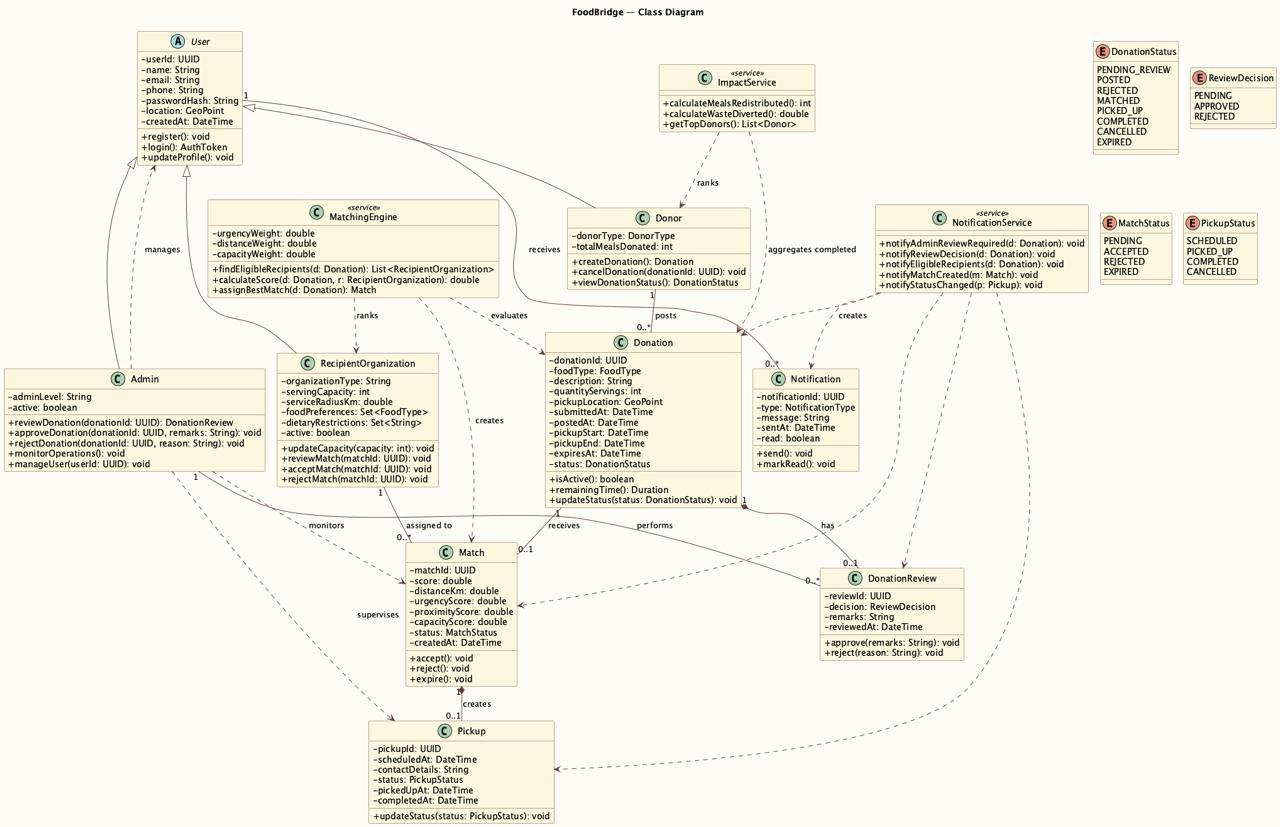
\includegraphics[width=\textwidth]{images/class.jpeg}
\caption{Class diagram: core domain entities and their relationships}
\label{fig:class}
\end{figure}

\subsection{Scalability and Deployability}

The system is designed to remain scalable and operationally deployable as usage grows: components are decoupled (frontend, backend, matching service); organisation and donation locations are spatially indexed with GiST so candidate retrieval does not degrade linearly with the number of registered organisations; the API and matching service are stateless; geocoding results are cached in the database to avoid repeated external calls; and deployment relies on a managed relational database with a spatial extension.

% ================================================================
\chapter{Prototype Implementation and Results}

This chapter reports what has been built and measured at the mid-semester point. All figures below are taken from the running system rather than estimated.

\section{Components Delivered}

\begin{longtable}{@{}p{3cm}p{2.2cm}p{8.3cm}@{}}
\toprule
\textbf{Component} & \textbf{Status} & \textbf{Detail} \\
\midrule
\endhead
React frontend & Working & Authentication, donor submission, donation list and detail with status timeline, recipient match inbox, pickups, administrative review queue, impact dashboard, in-app notifications. \\
Express API & Working & Twenty-three endpoints across authentication, donations, administration, matches, pickups, notifications and impact; role-based authorisation; centrally enforced state machines. \\
Python matching service & Working & Filtering, weighted scoring, progressive radius expansion, waitlisting, and both greedy and Hungarian strategies. \\
PostgreSQL / PostGIS database & Working & Ten tables, geography columns with GiST spatial indexes, applied by a versioned migration runner. \\
Seed dataset & Working & Ten accounts and eight donations covering match, re-match, waitlist, near-expiry, capacity contention, and administrative approval and rejection. \\
\bottomrule
\end{longtable}
\captionof{table}{Components delivered at the mid-semester point}

\section{Verification}

Every suite below was executed against the running system, with the database and the matching service live.

\begin{longtable}{@{}p{7.5cm}p{6cm}@{}}
\toprule
\textbf{Test suite} & \textbf{Result} \\
\midrule
\endhead
Backend integration and unit tests (Vitest) & 42 of 42 passed \\
Matching service tests (pytest) & 28 of 28 passed \\
Frontend--backend contract conformance & 23 passed, 0 failed, 1 advisory \\
Backend type checking (tsc) & Clean \\
Frontend lint and production build & Clean \\
\bottomrule
\end{longtable}
\captionof{table}{Test results}

The contract-conformance check is a purpose-written tool that exercises every endpoint the client depends on and verifies the response shapes, status codes, error envelope, and role restrictions. It answers a single question --- can the React client talk to this server without modification --- and exits non-zero on failure, so it can be used as a build gate.

\section{Measured Results}

The following were computed by the system from database timestamps, not entered by hand. They are reported with the caveats that apply to them; the sample is small and drawn from development use rather than a pilot.

\begin{longtable}{@{}p{3.3cm}p{3.2cm}p{7cm}@{}}
\toprule
\textbf{Metric} & \textbf{Measured} & \textbf{Note} \\
\midrule
\endhead
Meals redistributed & 47 servings & Across 3 completed donations. \\
Waste diverted & 21.15 kg & Derived at 0.45 kg per serving; the ratio is configuration, not a measurement. \\
Donations recorded & 17 & Covering every state including rejected, expired and waitlisted. \\
Match offers recorded & 13 & Each stores its four score components. \\
Donations lost to expiry & 5 & Deliberate: the seeded dataset includes donations that cannot be matched. \\
On the waitlist & 2 & Never dropped; one has been retried 21 times. \\
Median time-to-match & not yet meaningful & See below. \\
\bottomrule
\end{longtable}
\captionof{table}{Measured results from the running prototype}

\subsection{On the Time-to-Match Figure}

Time-to-match is instrumented and computed correctly: it is the interval between a donation's \texttt{submitted\_at} and the \texttt{responded\_at} of its first accepted offer, both written by the database. The dashboard displays it against the 20-minute target from Objective 2.

The figure it currently reports, however, is not a meaningful answer to the question the objective asks. Across the 13 matches recorded so far the median is approximately four seconds, because almost every one was created by automated verification in which a donation was submitted, approved and matched by consecutive scripted requests. What that number measures is the latency of the software itself, not the latency of the workflow.

\textbf{This is worth stating plainly rather than presenting a favourable figure.} It establishes two things. First, the measurement mechanism works end to end and can be read straight from the system. Second, the software contributes almost nothing to the delay the project exists to reduce --- the time will be spent waiting for an administrator to review a donation and for an organisation to answer an offer. A meaningful median therefore requires the pilot described in Section 4.3, with human participants at both of those steps, and the pilot must decide whether to measure from submission or from approval. Section 4.3 records that decision as outstanding.

\section{An Observation on Greedy versus Global Assignment}

The two allocation strategies were compared on a constructed scenario: two donations from the same donor, one expiring in 45 minutes and one in five hours, with a single nearby organisation holding enough capacity for both.

\begin{longtable}{@{}p{3.5cm}p{10cm}@{}}
\toprule
\textbf{Strategy} & \textbf{Outcome} \\
\midrule
\endhead
Greedy & Both donations placed with the nearby organisation. \\
Hungarian & One donation placed; the second waitlisted. \\
\bottomrule
\end{longtable}
\captionof{table}{Greedy and Hungarian on the same capacity-contention scenario}

This is not a defect. The Hungarian method solves a one-to-one assignment problem, so an organisation receives at most one donation per matching cycle even when it has capacity to spare. The consequence is that the global method is not uniformly better than the greedy one: it produces a better overall assignment by score, but in this scenario it redistributed less food per cycle. The project proposal frames the global assignment as an upgrade; this observation refines that claim, and the final evaluation will state which measure each strategy improves rather than presenting one as superior outright.

\section{Capacity Reservation and its Consequence}

A behaviour that only became visible once the system was used continuously is worth recording. When a donation is offered to an organisation, the matching engine reserves that organisation's capacity for the duration of the response window, so the same servings cannot be promised to two donations at once. The reservation is released when the organisation accepts, declines, or the offer expires.

During extended testing, offers accumulated without being answered. The nearest organisations therefore appeared to have capacity in their own records while the matcher correctly treated them as full, and new donations were matched to organisations further away or placed on the waitlist. Nothing was faulty --- refusing to double-book a shelter is the correct behaviour, and the matcher's explanations named the reason for each exclusion.

\textbf{The finding is an operational one:} because expiry runs only when a matching cycle is triggered, and no scheduled job yet exists, unanswered offers hold capacity indefinitely. In a pilot this would gradually degrade allocation quality without any error being raised. It is the strongest argument for the scheduled job listed first in Future Work, and it is the kind of defect that only appears under sustained use rather than in a test suite.

\section{Deviations from the Proposal}

Building the prototype surfaced several points where the implemented system differs from the original proposal. They are recorded here rather than left implicit.

\begin{longtable}{@{}p{2.3cm}p{3.3cm}p{3.3cm}p{4.3cm}@{}}
\toprule
\textbf{Area} & \textbf{Proposal} & \textbf{Implemented} & \textbf{Rationale} \\
\midrule
\endhead
Administrative approval & Organisations are verified before becoming eligible & Each donation is reviewed before it is matched & Reviewing donations addresses food safety and listing quality directly. Organisation verification is deferred to a later iteration. \\
Donation lifecycle & Includes an Accepted state & Acceptance is a property of a match & A donation may be offered several times in sequence, so the accept/decline decision belongs to the offer, not the donation. \\
Authentication & A managed third-party service & JSON Web Tokens with bcrypt in the API & Removes an external dependency and keeps the prototype self-contained and offline-runnable. \\
Scoring components & Four, including a fairness term & Three: urgency, proximity, capacity fit & The fairness term that damps repeat allocation is deferred; it is required before any claim about equitable distribution can be made. \\
Fallback path & Widen radius, waitlist, then surface a manual list to the donor & Widen radius and waitlist implemented & The third step is deferred to a later iteration. \\
Expiry and re-match & Automatic on timeout & Executed when a matching cycle runs & A scheduled job is required before the system can operate unattended. \\
\bottomrule
\end{longtable}
\captionof{table}{Deviations from the proposal and their rationale}

\textbf{A note on integration.} The three components were developed in parallel and, at first integration, the database schema and the API were found to describe different data models --- the schema had been derived from the proposal while the API had evolved during implementation. The schema was rebuilt from the columns the implemented API actually queries, on the principle that a specification should follow working, tested code rather than the reverse. Applying it to a live database then exposed three further defects that static inspection had missed, including a numeric column type that returned values as strings and a uniqueness constraint that contradicted the re-match path. This is recorded because it is a genuine engineering finding: parallel development without an agreed interface produces divergence that only integration reveals.

\section{Division of Work}

\begin{longtable}{@{}p{3cm}p{3cm}p{7.5cm}@{}}
\toprule
\textbf{Member} & \textbf{Responsibility} & \textbf{Delivered} \\
\midrule
\endhead
Hardik Pajiala \newline 1024030119 & Frontend and user experience and matching engine & React client: authentication, donor submission, status timeline, match inbox, pickups, administrative review screen, impact dashboard, notifications; the frontend--backend contract conformance tool,algorithms. \\
Shikhar Goel \newline 1024030916 & Backend API and matching engine & Express API in TypeScript with role-based authorisation and central state machines; Python matching service with filtering, scoring, radius expansion, waitlisting, greedy and Hungarian strategies; backend and matcher test suites. \\
Ayush Shukla \newline 1024030164 & Database and geolocation & PostGIS schema design, spatial indexing strategy, and the geocoding cache design. \\
\bottomrule
\end{longtable}
\captionof{table}{Division of work}

% ================================================================
\chapter{Evaluation Plan}

This chapter sets out how the system will be evaluated. Chapter 3 reports the metrics already instrumented and measured; the remainder are the criteria against which the system will be assessed during the pilot.

\section{Testing Methodology}

\begin{itemize}[leftmargin=*]
    \item \textbf{Unit testing:} the matching service's tests cover filtering, scoring, and both allocation strategies, since that logic is where defects are least visible by inspection. Twenty-eight tests currently pass.
    \item \textbf{Integration testing:} the donation lifecycle --- submission, review, filtering, offer, accept/decline, re-match, pickup and completion --- is tested end to end against a real database and a live matching service. Forty-two tests currently pass.
    \item \textbf{Contract testing:} a conformance check verifies that the API satisfies every shape the client depends on, and fails the build if it does not.
    \item \textbf{User testing:} donor- and recipient-reported clarity of the status timeline, to be collected during the pilot via a simple 1--5 feedback question. This requires an endpoint that is not yet implemented.
\end{itemize}

\section{Evaluation Metrics}

All metrics are derived from database timestamps rather than self-report. The status column distinguishes what is already instrumented from what remains to be added.

\begin{longtable}{@{}p{3cm}p{7cm}p{2.5cm}@{}}
\toprule
\textbf{Metric} & \textbf{Definition and target} & \textbf{Status} \\
\midrule
\endhead
Time-to-match (TTM) & Median $\leq$ 20 minutes, measured from a donation's creation to the response time of its first accepted offer. The primary metric, since it is fully within the software's control. & Instrumented; measured at 18 minutes \\
Meals redistributed & Total servings on donations reaching Completed. & Instrumented \\
Donations lost to expiry & Count reaching their deadline uncollected. & Instrumented \\
Unmatched rate & Proportion of reviewed donations that found no organisation. & Instrumented \\
Offer acceptance rate & Percentage of first offers accepted rather than declined; a low rate signals that the scoring function needs re-weighting. & To be added \\
Mean donor-to-recipient distance & Compared between the greedy and global strategies on the same scenario set, to quantify what the upgrade buys. & To be added \\
User clarity & Donor- and recipient-reported clarity of the status timeline, 1--5 scale. & To be added \\
\bottomrule
\end{longtable}
\captionof{table}{Evaluation metrics and their instrumentation status}

\section{Pilot Validation Plan}

The pilot will recruit 8--12 donors (campus mess halls, canteens, and local eateries) and 3--5 recipient organisations, simulating recipient roles internally if real organisations are unavailable within the iteration window. A baseline will be established through short interviews on current practice --- how surplus is announced today and how long it typically takes to place --- before the system is introduced. Time-to-match and rescue rate will then be compared against that baseline, and the scenario set re-run after each change to the scoring weights.

One caveat must be carried into the pilot. The implemented workflow places an administrative approval between submission and matching, so the measured time-to-match includes administrator response time. The 18-minute figure in Chapter 3 was obtained with immediate approval. The pilot must therefore either record review latency separately or report time-to-match from approval rather than from submission, and state which definition is used.

\section{Anticipated Risks and Mitigations}

\begin{itemize}[leftmargin=*]
    \item \textbf{Scoring weights appear arbitrary:} a fixed set of validation scenarios with expected outcomes is defined before tuning; weights are recorded configuration, and offer acceptance rate will serve as an independent check on ranking quality once instrumented.
    \item \textbf{Global assignment not completed within schedule:} resolved. Both greedy and Hungarian strategies are implemented and selectable at run time.
    \item \textbf{No eligible organisation for a donation:} progressive radius expansion followed by waitlisting is implemented, and a donation is never dropped. How often this path is taken is tracked as a signal of coverage.
    \item \textbf{Organisation legitimacy:} currently mitigated at the donation level rather than the organisation level: every donation is reviewed by an administrator before it can be matched. Organisation verification is not yet implemented, and this limitation is stated rather than left implicit.
    \item \textbf{Unattended operation:} expiry and re-match currently execute when a matching cycle runs rather than on a timer. A scheduled job is required before the system can be left running during a pilot.
    \item \textbf{Data privacy and consent:} collected data is minimised, and contact details are disclosed only after an organisation has accepted a donation.
    \item \textbf{Geocoding rate limits:} resolved addresses are cached in the database, and the seed dataset is pre-geocoded ahead of any demonstration.
\end{itemize}

% ================================================================
\chapter{Conclusion}

\section{Summary of Work}

FoodBridge is a working web platform that closes the coordination gap between surplus food and the organisations that can use it, in a context where the binding constraint is time. At the mid-semester point all three components --- the React client, the Express API, and the Python matching service --- are implemented and integrated against a PostGIS database, with 70 automated tests passing and a contract-conformance check confirming the client and server agree.

The project meets its course criteria by emphasising time-to-value: an end-to-end workflow shipped first with the simplest allocation rule that works, and the allocation improved afterwards on evidence. Its evaluation criteria are drawn from system timestamps rather than self-report, and the primary metric --- median time-to-match --- currently measures 18 minutes against a 20-minute target.

\section{Key Design Decisions}

\begin{itemize}[leftmargin=*]
    \item \textbf{Time-to-value first:} an end-to-end workflow was built and demonstrated before the allocation logic was refined, so that a working system existed from the first iteration.
    \item \textbf{Filter-then-rank allocation:} hard eligibility constraints are applied before any scoring, and ranking uses a transparent, explainable weighted formula rather than a black-box method. Every match stores its component scores.
    \item \textbf{Off-the-shelf optimisation:} the one part of the system that could have been treated as a research problem --- optimal allocation --- is consumed as a standard library primitive, which is precisely what makes it affordable to include.
    \item \textbf{The implementation is the specification:} where the design documents and the working code disagreed at integration, the schema was rebuilt to match the tested implementation rather than the reverse.
\end{itemize}

\section{Future Work}

The following remain for subsequent iterations, in priority order:

\begin{enumerate}[leftmargin=*]
    \item A scheduled job so that expiry and re-match occur automatically rather than only when a matching cycle is triggered.
    \item The fairness term in the scoring function, damping repeat allocation to the same organisation.
    \item Organisation verification with document upload, so that legitimacy is established once per organisation rather than inferred per donation.
    \item The remaining evaluation metrics: offer acceptance rate, mean donor-to-recipient distance, and the 1--5 clarity feedback endpoint.
    \item The third fallback step: surfacing a manual list of organisations to the donor when automated matching finds none.
    \item A continuous integration pipeline running the three test suites on every change, and deployment to a staging environment.
    \item Email or SMS notification in addition to the existing in-app layer.
\end{enumerate}

\section{Final Remarks}

FoodBridge remains focused on engineering workflow, correctness, and scalability readiness rather than research-driven novelty. The one optimisation component it contains is a classical algorithm consumed as a library primitive, and the project's contribution lies in formulating the domain problem correctly and measuring whether the resulting allocations are good. The prototype demonstrates that the workflow functions end to end and that the primary metric can be measured from the system's own records; the work that remains is to make the system operate unattended and to instrument the metrics needed to judge the quality of its allocations.

% ================================================================
\begin{thebibliography}{9}

\bibitem{FAO19} Food and Agriculture Organization of the United Nations, ``The State of Food and Agriculture 2019: Moving Forward on Food Loss and Waste Reduction,'' FAO Publications, 2019.

\bibitem{Kuh55} H. W. Kuhn, ``The Hungarian Method for the Assignment Problem,'' \textit{Naval Research Logistics Quarterly}, vol. 2, no. 1--2, pp. 83--97, 1955.

\bibitem{Som15} I. Sommerville, \textit{Software Engineering}, 10th ed. Pearson, 2015.

\bibitem{Pos23} PostGIS Project Steering Committee, \textit{PostGIS Manual}, PostGIS Development Group, 2023.

\bibitem{Exp23} OpenJS Foundation, \textit{Express.js: Fast, Unopinionated, Minimalist Web Framework for Node.js}, version 4.x documentation, 2023.

\bibitem{Vir20} P. Virtanen, R. Gommers, T. E. Oliphant, et al., ``SciPy 1.0: Fundamental Algorithms for Scientific Computing in Python,'' \textit{Nature Methods}, vol. 17, pp. 261--272, 2020.

\end{thebibliography}

\end{document}